\documentclass{cmn}

\begin{document}
  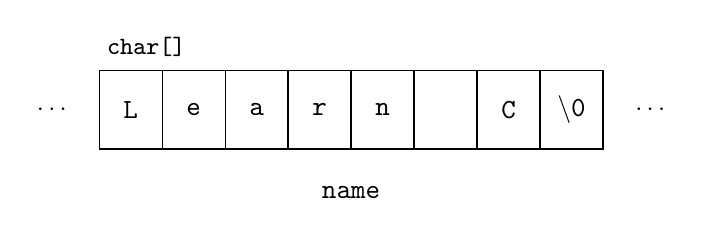
\begin{tikzpicture}
    \draw (-3*8mm,0) -- ++(8*8mm,0) -- ++(0,10mm) -- ++(-8*8mm,0) -- cycle;
    \foreach \i in {-2,...,4} {
      \draw (\i*8mm,0) -- ++(0,10mm);
    }

    \node at (-3*8mm-6mm,5mm) {\small$\cdots$};
    \node at (5*8mm+6mm,5mm) {\small$\cdots$};

    \foreach \i/\t in {-2/L,-1/e,0/a,1/r,2/n,4/C,5/{\textbackslash}0} {
      \node at (\i*8mm-4mm,5mm) {\texttt{\t}};
    }

    \node at (-3*8mm+6mm,10mm+3mm) {\small\texttt{char[]}};
    \node at (8mm,-5.5mm) {\texttt{name}};
  \end{tikzpicture}
\end{document}
